% EGE 2027, task 10. Source IDs and URLs are kept in comments.
% Editable task bank. Append new BankTask blocks at the end of the document.
\documentclass[12pt,a4paper]{article}
\usepackage{physics-textbook}
\usepackage{graphicx,needspace}
\newif\ifShowSolutions
\ifdefined\TutorEdition
  \ShowSolutionstrue
\else
  \ShowSolutionsfalse
\fi
\newcounter{banktask}
\newcommand{\BankTask}[3]{%
  \refstepcounter{banktask}%
  \Needspace{35mm}\par\medskip\noindent\begin{minipage}{\linewidth}%
  \noindent\textbf{\thebanktask.}\quad #2\par
  \ifShowSolutions
    #3\par
    \ifdefined\TutorEdition
      \ifcsname TutorSource#1\endcsname
        \smallskip{\small\csname TutorSource#1\endcsname\par}%
      \fi
    \fi
  \fi
  \end{minipage}\par\medskip
}
\begin{document}
Справочные величины (если в условии не оговорено иное):\par
$R=8{,}31\,\text{Дж}/(\text{моль}\cdot\text{К})$\par
$M_{\mathrm{Ar}}=40\,\text{г}/\text{моль}$



% Source 5644DE: https://ege.fipi.ru/bank/questions.php?search=1&proj=BA1F39653304A5B041B656915DC36B38&qid=5644DE
\BankTask{5644DE}{
В цилиндре под поршнем находится идеальный одноатомный газ. Формулы А и Б позволяют рассчитать значения физических величин, характеризующих состояние газа. Использованы обозначения: \(p\) — давление; \(V\) — объём; \(\overline{E}_{\text{к}}\) — средняя кинетическая энергия поступательного теплового движения частиц газа; \(\nu\) — количество вещества, \(N_A\) — постоянная Авогадро.

Установите соответствие между формулами и физическими величинами, значение которых можно рассчитать по этим формулам.

\begin{center}
\TaskMatchingColumns[.35\linewidth]{Формулы}{
А) \(\displaystyle\frac{2}{3}\frac{\nu N_A\overline{E}_{\text{к}}}{V}\)\par
Б) \(\displaystyle\frac{3}{2}\frac{pV}{N_A\overline{E}_{\text{к}}}\)
}{Физические величины}{
1) масса газа\par
2) количество вещества\par
3) давление\par
4) абсолютная температура
}

\begin{tabular}{|c|c|}
\hline
А & Б \\
\hline
\phantom{0} & \phantom{0} \\
\hline
\end{tabular}
\end{center}
}{
\smallskip\noindent\textbf{Решение от GPT}\par
Основное уравнение МКТ: \(pV=\frac{2}{3}N\overline{E}_{\text{к}}\), где \(N=\nu N_A\). Поэтому \(p=\frac{2}{3}\frac{\nu N_A\overline{E}_{\text{к}}}{V}\): А — 3. Выражая количество вещества, получаем \(\nu=\frac{3}{2}\frac{pV}{N_A\overline{E}_{\text{к}}}\): Б — 2.

Ответ: А — 3, Б — 2; \(32\).
}

% Source CD1D80: https://ege.fipi.ru/bank/questions.php?search=1&proj=BA1F39653304A5B041B656915DC36B38&qid=CD1D80
\BankTask{CD1D80}{
В цилиндре под поршнем находится идеальный одноатомный газ. Формулы А и Б позволяют рассчитать значения физических величин, характеризующих состояние газа. Обозначения: \(p\) — давление; \(T\) — абсолютная температура; \(N\) — число атомов газа; \(k\) — постоянная Больцмана, \(V\) — объём газа.

Установите соответствие между формулами и физическими величинами, значение которых можно рассчитать по этим формулам.

\begin{center}
\TaskMatchingColumns[.35\linewidth]{Формулы}{
А) \(\displaystyle\frac{p}{kT}\)\par
Б) \(\displaystyle\frac{pV}{Nk}\)
}{Физические величины}{
1) абсолютная температура\par
2) концентрация молекул\par
3) давление\par
4) внутренняя энергия
}

\begin{tabular}{|c|c|}
\hline
А & Б \\
\hline
\phantom{0} & \phantom{0} \\
\hline
\end{tabular}
\end{center}
}{
\smallskip\noindent\textbf{Решение от GPT}\par
Из \(p=nkT\) следует \(n=\frac{p}{kT}\), то есть формула А определяет концентрацию молекул: А — 2. Из \(pV=NkT\) получаем \(T=\frac{pV}{Nk}\), то есть формула Б определяет абсолютную температуру: Б — 1.

Ответ: А — 2, Б — 1; \(21\).
}

% Source B5F219: https://ege.fipi.ru/bank/questions.php?search=1&proj=BA1F39653304A5B041B656915DC36B38&qid=B5F219
\BankTask{B5F219}{
Одноатомный идеальный газ в количестве \(0{,}04\,\text{моль}\), находящийся в сосуде под подвижным поршнем, изотермически расширяется при температуре \(450\,\text{К}\). Масса газа в сосуде остаётся неизменной.

Установите соответствие между физическими величинами, характеризующими газ, и формулами, выражающими их зависимость от объёма \(V\) газа.

\begin{center}
\TaskMatchingColumns[.53\linewidth]{Физические величины}{
А) давление газа \(p(V)\)\par
Б) внутренняя энергия газа \(U(V)\)
}{Формулы}{
1) \(18\cdot V\)\par
2) \(\displaystyle\frac{149{,}58}{V}\)\par
3) \(224{,}37\)\par
4) \(27\)
}

\begin{tabular}{|c|c|}
\hline
А & Б \\
\hline
\phantom{0} & \phantom{0} \\
\hline
\end{tabular}
\end{center}
}{
\smallskip\noindent\textbf{Решение от GPT}\par
При \(R=8{,}31\,\text{Дж}/(\text{моль}\cdot\text{К})\) имеем \(\nu RT=0{,}04\cdot8{,}31\cdot450=149{,}58\,\text{Дж}\). По уравнению состояния \(p(V)=\frac{\nu RT}{V}=\frac{149{,}58}{V}\) (давление в паскалях при объёме в \(\text{м}^3\)): А — 2. Внутренняя энергия одноатомного газа \(U=\frac{3}{2}\nu RT=224{,}37\,\text{Дж}\) постоянна: Б — 3.

Ответ: А — 2, Б — 3; \(23\).
}

% Source 65ACC9: https://ege.fipi.ru/bank/questions.php?search=1&proj=BA1F39653304A5B041B656915DC36B38&qid=65ACC9
\BankTask{65ACC9}{
Аргон в количестве $\nu\,\text{моль}$ помещают в открытый сверху сосуд под тяжёлый подвижный поршень и начинают охлаждать. Начальное давление газа — $p_0$. Трением между поршнем и стенками сосуда пренебречь.

Установите соответствие между физическими величинами, характеризующими газ, и формулами, выражающими их зависимость от абсолютной температуры $T$ газа ($R$ — универсальная газовая постоянная).

\begin{center}
\TaskMatchingColumns[.53\linewidth]{Физические величины}{
А) объём газа $V(T)$\par
Б) внутренняя энергия газа $U(T)$
}{Формулы}{
1) $\dfrac{\nu RT}{p_0}$\par
2) $\dfrac{\nu Rp_0}{T}$\par
3) $\dfrac{3}{2}\nu RT$\par
4) $\dfrac{3}{2}\dfrac{\nu RT}{p_0}$
}
\end{center}

\begin{center}
\begin{tabular}{|c|c|}\hline
А & Б \\ \hline
\phantom{00} & \phantom{00} \\ \hline
\end{tabular}
\end{center}
}{
\smallskip\noindent\textbf{Решение от GPT}\par
Тяжёлый подвижный поршень поддерживает постоянное давление $p=p_0$. Из уравнения состояния $p_0V=\nu RT$ получаем $V(T)=\dfrac{\nu RT}{p_0}$: А — 1. Аргон — одноатомный идеальный газ, поэтому $U(T)=\dfrac{3}{2}\nu RT$: Б — 3.

Ответ: А — 1, Б — 3.
}

% Source 8054C4: https://ege.fipi.ru/bank/questions.php?search=1&proj=BA1F39653304A5B041B656915DC36B38&qid=8054C4
\BankTask{8054C4}{
Аргон массой $160\,\text{г}$ при комнатной температуре помещают в герметичный закрытый сосуд объёмом $20\,\text{л}$ и начинают нагревать. Масса газа в сосуде остаётся неизменной.

Установите соответствие между физическими величинами, характеризующими аргон, и формулами, выражающими их зависимость от абсолютной температуры $T$ газа в условиях данной задачи.

\begin{center}
\TaskMatchingColumns[.53\linewidth]{Физические величины}{
А) давление газа $p(T)$\par
Б) внутренняя энергия газа $U(T)$
}{Формулы}{
1) $aT$, $a=1662\,\dfrac{\text{Па}}{\text{К}}$\par
2) $bT$, $b=49{,}86\,\dfrac{\text{Дж}}{\text{К}}$\par
3) $\dfrac{c}{T}$, $c=80\,\text{Дж}\cdot\text{К}$\par
4) $dT$, $d=4{,}986\,\dfrac{\text{Па}}{\text{К}}$
}
\end{center}

\begin{center}
\begin{tabular}{|c|c|}\hline
А & Б \\ \hline
\phantom{00} & \phantom{00} \\ \hline
\end{tabular}
\end{center}
}{
\smallskip\noindent\textbf{Решение от GPT}\par
Используем молярную массу аргона $M=40\,\text{г/моль}$. Тогда $\nu=m/M=4\,\text{моль}$, $V=0{,}020\,\text{м}^3$.
\[
p(T)=\frac{\nu R}{V}T=\left(1662\,\frac{\text{Па}}{\text{К}}\right)T,
\qquad
U(T)=\frac32\nu RT=\left(49{,}86\,\frac{\text{Дж}}{\text{К}}\right)T.
\]
Давлению соответствует формула 1, внутренней энергии одноатомного газа — формула 2.

Ответ: А — 1, Б — 2.
}

% Source D67CAF: https://ege.fipi.ru/bank/questions.php?search=1&proj=BA1F39653304A5B041B656915DC36B38&qid=D67CAF
\BankTask{D67CAF}{
Температура нагревателя идеального теплового двигателя, работающего по циклу Карно, равна $T_1$, а коэффициент полезного действия этого двигателя равен $\eta$. За цикл рабочее тело двигателя получает от нагревателя количество теплоты $Q_1$.

Установите соответствие между физическими величинами и формулами, по которым их можно рассчитать.

\TaskMatchingColumns[0.58\linewidth]{Физические величины}{
А) количество теплоты, отдаваемое рабочим телом двигателя за цикл\par
Б) температура холодильника
}{Формулы}{
1) $\dfrac{T_1}{1-\eta}$\par
2) $T_1(1-\eta)$\par
3) $Q_1(1-\eta)$\par
4) $Q_1\eta$
}

\begin{center}
\begin{tabular}{|c|c|}\hline
А & Б \\ \hline
\phantom{00} & \phantom{00} \\ \hline
\end{tabular}
\end{center}
}{
\smallskip\noindent\textbf{Решение от GPT}\par
Обозначим отданное холодильнику количество теплоты через $Q_2>0$. Из $\eta=\dfrac{Q_1-Q_2}{Q_1}$ следует $Q_2=Q_1(1-\eta)$: А — 3. Для цикла Карно $\eta=1-\dfrac{T_2}{T_1}$, поэтому $T_2=T_1(1-\eta)$: Б — 2.

Ответ: А — 3, Б — 2.
}

% Source A53641: https://ege.fipi.ru/bank/questions.php?search=1&proj=BA1F39653304A5B041B656915DC36B38&qid=A53641
\BankTask{A53641}{
\begin{center}
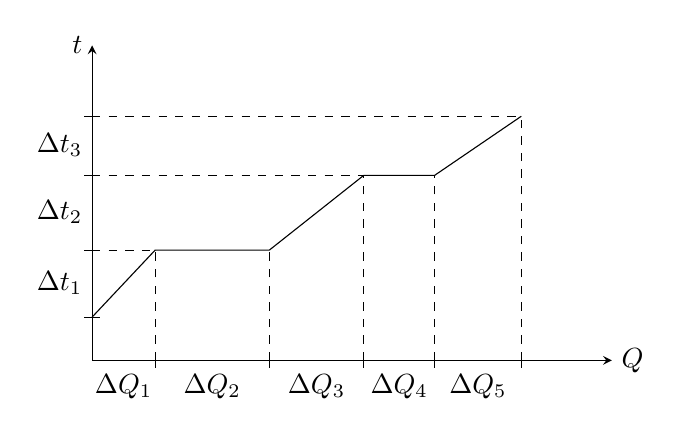
\begin{tikzpicture}[x=1cm,y=1cm,>=stealth]
\draw[->] (0,0)--(6.6,0) node[right] {$Q$};
\draw[->] (0,0)--(0,4) node[left] {$t$};
\draw (0,0.55)--(0.8,1.4)--(2.25,1.4)--(3.45,2.35)--(4.35,2.35)--(5.45,3.1);
\foreach \x/\y in {0.8/1.4,2.25/1.4,3.45/2.35,4.35/2.35,5.45/3.1} {
\draw[dashed] (\x,0)--(\x,\y);
\draw (\x,0.1)--(\x,-0.1);
}
\foreach \y in {0.55,1.4,2.35,3.1} {\draw (-0.1,\y)--(0.1,\y);}
\draw[dashed] (0,1.4)--(0.8,1.4);
\draw[dashed] (0,2.35)--(3.45,2.35);
\draw[dashed] (0,3.1)--(5.45,3.1);
\node[left] at (0,0.98) {$\Delta t_1$};
\node[left] at (0,1.88) {$\Delta t_2$};
\node[left] at (0,2.73) {$\Delta t_3$};
\node[below] at (0.4,-0.06) {$\Delta Q_1$};
\node[below] at (1.525,-0.06) {$\Delta Q_2$};
\node[below] at (2.85,-0.06) {$\Delta Q_3$};
\node[below] at (3.9,-0.06) {$\Delta Q_4$};
\node[below] at (4.9,-0.06) {$\Delta Q_5$};
\end{tikzpicture}
\end{center}
В цилиндре под поршнем находилось твёрдое вещество массой $m$. Цилиндр поместили в печь. На рисунке схематично показан график изменения температуры $t$ вещества по мере поглощения им количества теплоты $Q$. Формулы А и Б позволяют рассчитать значения физических величин, характеризующих происходящие с веществом тепловые процессы.

Установите соответствие между формулами и физическими величинами, значение которых можно рассчитать по этим формулам.



\begin{center}
\TaskMatchingColumns[.35\linewidth]{Формулы}{
А) $\displaystyle\frac{\Delta Q_1}{m\Delta t_1}$\par
Б) $\displaystyle\frac{\Delta Q_2}{m}$
}{Физические величины}{
1) удельная теплота плавления\par
2) удельная теплота парообразования\par
3) удельная теплоёмкость твёрдого вещества\par
4) удельная теплоёмкость жидкости
}

\begin{tabular}{|c|c|}
\hline
А & Б \\
\hline
\phantom{3} & \phantom{1} \\
\hline
\end{tabular}
\end{center}
}{
\smallskip\noindent\textbf{Решение от GPT}\par
А: первый наклонный участок соответствует нагреванию твёрдого вещества. Из $\Delta Q_1=mc_{\text{тв}}\Delta t_1$ получаем $c_{\text{тв}}=\dfrac{\Delta Q_1}{m\Delta t_1}$, поэтому А~--- 3.

Б: первый горизонтальный участок соответствует плавлению при постоянной температуре. Из $\Delta Q_2=\lambda m$ получаем $\lambda=\dfrac{\Delta Q_2}{m}$, поэтому Б~--- 1.

Ответ: $31$.
}

% Source F5A444: https://ege.fipi.ru/bank/questions.php?search=1&proj=BA1F39653304A5B041B656915DC36B38&qid=F5A444
\BankTask{F5A444}{
Один моль одноатомного идеального газа участвует в процессе $1$--$2$--$3$, график которого изображён на рисунке в координатах $p$--$T$, где $p$~--- давление газа, $T$~--- абсолютная температура газа. Как изменяются объём газа $V$ в ходе процесса $1$--$2$ и плотность газа $\rho$ в ходе процесса $2$--$3$?

\begin{center}
\begin{tikzpicture}[x=1cm,y=1cm,>=stealth]
\draw[->] (0,0)--(4,0) node[below] {$T$};
\draw[->] (0,0)--(0,3.3) node[left] {$p$};
\node[below left] at (0,0) {$0$};
\draw (0,0)--(2.9,1.22)--(2.9,3.05);
\fill (1.03,0.433) circle (1.2pt) node[above left] {$1$};
\fill (2.9,1.22) circle (1.2pt) node[right] {$2$};
\fill (2.9,3.05) circle (1.2pt) node[right] {$3$};
\draw[->] (1.4,0.589)--(1.95,0.82);
\draw[->] (2.9,1.7)--(2.9,2.2);
\end{tikzpicture}
\end{center}
Для каждой величины определите соответствующий характер изменения:

\begin{enumerate}
\item увеличивается
\item уменьшается
\item не изменяется
\end{enumerate}


\TaskChangeTable{Объём газа в ходе процесса $1$--$2$}{Плотность газа в ходе процесса $2$--$3$}
}{
\smallskip\noindent\textbf{Решение от GPT}\par
Из $pV=\nu RT$ следует $V=\nu RT/p$. На участке $1$--$2$ прямая проходит через начало координат, поэтому $p/T=\mathrm{const}$ и объём не изменяется (3).

На участке $2$--$3$ температура постоянна, давление увеличивается, поэтому объём уменьшается. При постоянной массе $\rho=m/V$ увеличивается (1).

Ответ: $31$.
}

% Source F0D87A: https://ege.fipi.ru/bank/questions.php?search=1&proj=BA1F39653304A5B041B656915DC36B38&qid=F0D87A
\BankTask{F0D87A}{
$1$ моль одноатомного идеального газа участвует в процессе $1$--$2$--$3$, график которого изображён на рисунке в координатах $p$--$V$, где $p$~--- давление газа, $V$~--- объём газа. Как изменяются концентрация молекул $n$ газа в ходе процесса $1$--$2$ и абсолютная температура $T$ газа в ходе процесса $2$--$3$? Масса газа остаётся постоянной.

\begin{center}
\begin{tikzpicture}[x=1cm,y=1cm,>=stealth]
\draw[->] (0,0)--(4.2,0) node[below] {$V$};
\draw[->] (0,0)--(0,3.5) node[left] {$p$};
\node[below left] at (0,0) {$0$};
\draw (0.8,0.9)--(3.2,0.9)--(3.2,2.9);
\fill (0.8,0.9) circle (1.2pt) node[below left] {$1$};
\fill (3.2,0.9) circle (1.2pt) node[below right] {$2$};
\fill (3.2,2.9) circle (1.2pt) node[above right] {$3$};
\draw[->] (1.4,0.9)--(2,0.9);
\draw[->] (3.2,1.4)--(3.2,1.95);
\end{tikzpicture}
\end{center}
Для каждой величины определите соответствующий характер изменения:

\begin{enumerate}
\item увеличивается
\item уменьшается
\item не изменяется
\end{enumerate}

\TaskChangeTable{Концентрация молекул газа в ходе процесса $1$--$2$}{Абсолютная температура газа в ходе процесса $2$--$3$}
}{
\smallskip\noindent\textbf{Решение от GPT}\par
На участке $1$--$2$ объём увеличивается. Число молекул $N$ постоянно, поэтому концентрация $n=N/V$ уменьшается (2).

На участке $2$--$3$ объём постоянен, давление увеличивается. Из $T=pV/(\nu R)$ следует, что температура увеличивается (1).

Ответ: $21$.
}

% Source F12DcD: https://ege.fipi.ru/bank/questions.php?search=1&proj=BA1F39653304A5B041B656915DC36B38&qid=F12DcD
\BankTask{F12DcD}{
\begin{center}
\begin{tikzpicture}[>=stealth,scale=0.85]
\draw[->] (0,0)--(4,0) node[below] {$T$};
\draw[->] (0,0)--(0,3.8) node[left] {$V$};
\node[below left] at (0,0) {$0$};
\coordinate (A) at (2.5,3.2);
\coordinate (B) at (2.5,1);
\coordinate (C) at (1.3,0.52);
\draw[dashed] (0,0)--(C);
\draw (A)--(B)--(C);
\draw[->] (2.5,2.65)--(2.5,1.95);
\draw[->] (2.25,0.9)--(1.75,0.7);
\fill (A) circle (1.5pt) node[right] {$1$};
\fill (B) circle (1.5pt) node[right] {$2$};
\fill (C) circle (1.5pt) node[above left] {$3$};
\end{tikzpicture}
\end{center}
Один моль идеального газа участвует в процессе \(1\text{–}2\text{–}3\), график которого изображён на рисунке в координатах \(V\text{–}T\), где \(V\) — объём газа, \(T\) — абсолютная температура газа. Как изменяются давление газа \(p\) в ходе процесса \(1\text{–}2\) и концентрация молекул газа \(n\) в ходе процесса \(2\text{–}3\)? Масса газа остаётся постоянной.

Для каждой величины определите соответствующий характер изменения:
\begin{enumerate}
\item увеличивается
\item уменьшается
\item не изменяется
\end{enumerate}
\TaskChangeTable{Давление газа в ходе процесса \(1\text{–}2\)}{Концентрация молекул газа в ходе процесса \(2\text{–}3\)}
}{
\smallskip\noindent\textbf{Решение от GPT}\par
В процессе \(1\text{–}2\) температура постоянна, а объём уменьшается. Из \(p=\nu RT/V\) следует, что давление увеличивается (\(1\)). В процессе \(2\text{–}3\) объём уменьшается при постоянном числе молекул, поэтому концентрация \(n=N/V\) увеличивается (\(1\)).

Ответ: \(11\).
}

% Source 298FF1: https://ege.fipi.ru/bank/questions.php?search=1&proj=BA1F39653304A5B041B656915DC36B38&qid=298FF1
\BankTask{298FF1}{
\begin{center}
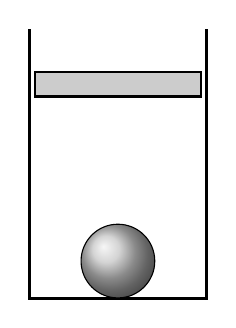
\begin{tikzpicture}[>=stealth,scale=0.9]
\draw[line width=1.2pt] (0,3.8)--(0,0)--(2.5,0)--(2.5,3.8);
\filldraw[fill=gray!40,line width=0.9pt] (0.08,2.85) rectangle (2.42,3.2);
\shade[ball color=gray!45] (1.25,0.53) circle (0.52);
\draw (1.25,0.53) circle (0.52);
\end{tikzpicture}
\end{center}
В цилиндрическом сосуде под поршнем находится газ. Поршень не закреплён и может перемещаться в сосуде без трения. На дне сосуда лежит стальной шарик (см. рисунок). Газ нагревают. Как изменятся в результате этого давление газа и действующая на шарик сила Архимеда? Атмосферное давление неизменно.

Для каждой величины определите соответствующий характер изменения:
\begin{enumerate}
\item увеличится
\item уменьшится
\item не изменится
\end{enumerate}
\TaskChangeTable{Давление газа}{Сила Архимеда}
}{
\smallskip\noindent\textbf{Решение от GPT}\par
Равновесие свободного поршня даёт \(p=p_{\text{атм}}+Mg/S\), где \(M\) — масса поршня, \(S\) — его площадь. Поэтому давление не изменится (\(3\)). При нагревании газ расширяется, его плотность \(\rho\) уменьшается. Следовательно, сила Архимеда \(F_A=\rho gV_{\text{ш}}\) уменьшится (\(2\)).

Ответ: \(32\).
}

% Source 28120c: https://ege.fipi.ru/bank/questions.php?search=1&proj=BA1F39653304A5B041B656915DC36B38&qid=28120c
\BankTask{28120c}{
\begin{center}
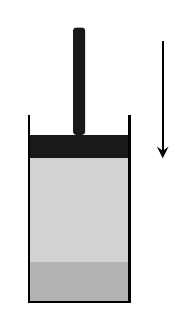
\begin{tikzpicture}[>=stealth,scale=0.85]
\fill[gray!35] (0,0.6) rectangle (1.5,2.15);
\fill[gray!60] (0,0) rectangle (1.5,0.6);
\fill[black!90] (0,2.15) rectangle (1.5,2.5);
\fill[black!90,rounded corners=1pt] (0.66,2.5) rectangle (0.84,4.1);
\draw[line width=0.9pt] (0,2.8)--(0,0)--(1.5,0)--(1.5,2.8);
\draw[->,line width=0.8pt] (2,3.9)--(2,2.15);
\end{tikzpicture}
\end{center}
В цилиндре под поршнем находятся жидкость и её насыщенный пар (см. рисунок). Как изменятся давление и концентрация молекул пара при медленном перемещении поршня вниз, если температура останется неизменной? В процессе движения поршень не касается поверхности жидкости.

Для каждой величины определите соответствующий характер изменения:
\begin{enumerate}
\item увеличится
\item уменьшится
\item не изменится
\end{enumerate}
\TaskChangeTable{Давление пара}{Концентрация молекул пара}
}{
\smallskip\noindent\textbf{Решение от GPT}\par
При медленном изотермическом сжатии часть насыщенного пара конденсируется. Пока присутствуют жидкость и пар, давление \(p_{\text{нас}}(T)\) при неизменной температуре постоянно (\(3\)). Из \(n=p_{\text{нас}}/(kT)\) следует, что концентрация молекул пара также не изменяется (\(3\)).

Ответ: \(33\).
}

% Source C427F7: https://ege.fipi.ru/bank/questions.php?search=1&proj=BA1F39653304A5B041B656915DC36B38&qid=C427F7
\BankTask{C427F7}{
Объём сосуда с идеальным газом уменьшили вдвое, выпустив половину газа и поддерживая температуру газа в сосуде постоянной. Как изменились при этом давление газа в сосуде и его внутренняя энергия?

Для каждой величины определите соответствующий характер изменения:

\begin{enumerate}
\item увеличилась
\item уменьшилась
\item не изменилась
\end{enumerate}


\TaskChangeTable{Давление газа в сосуде}{Внутренняя энергия газа в сосуде}
}{
\smallskip\noindent\textbf{Решение от GPT}\par
При постоянной температуре \(p=\nu RT/V\). Поскольку \(\nu_2=\nu_1/2\) и \(V_2=V_1/2\), получаем \(p_2=p_1\): давление не изменилось (\(3\)). Внутренняя энергия идеального газа при неизменной температуре пропорциональна количеству вещества: \(U_2=U_1/2\), поэтому она уменьшилась (\(2\)).

Ответ: \(32\).
}

% Source FB5B0D: https://ege.fipi.ru/bank/questions.php?search=1&proj=BA1F39653304A5B041B656915DC36B38&qid=FB5B0D
\BankTask{FB5B0D}{
В сосуде неизменного объёма при комнатной температуре находилась смесь неона и аргона, по \(2\,\text{моль}\) каждого. Половину смеси выпустили, а затем добавили в сосуд \(2\,\text{моль}\) аргона. Как в результате этого изменились парциальное давление аргона и давление смеси газов, если температура смеси оставалась неизменной? Для каждой величины определите соответствующий характер изменения:

\begin{enumerate}
\item увеличилась
\item уменьшилась
\item не изменилась
\end{enumerate}


\TaskChangeTable{Парциальное давление аргона}{Давление смеси газов в сосуде}
}{
\smallskip\noindent\textbf{Решение от GPT}\par
После выпуска половины смеси осталось по \(1\,\text{моль}\) каждого газа. После добавления аргона \(\nu_{\mathrm{Ar},2}=3\,\text{моль}\), а общее количество вещества \(\nu_2=4\,\text{моль}\). При постоянных \(T\) и \(V\) давление пропорционально количеству вещества. Поэтому парциальное давление аргона увеличилось в \(3/2\) раза (\(1\)), а давление смеси не изменилось, поскольку первоначально также было \(4\,\text{моль}\) газа (\(3\)).

Ответ: \(13\).
}

% Source 1D2B0A: https://ege.fipi.ru/bank/questions.php?search=1&proj=BA1F39653304A5B041B656915DC36B38&qid=1D2B0A
\BankTask{1D2B0A}{
Постоянная масса одноатомного идеального газа в изохорном процессе отдаёт количество теплоты \(Q>0\). Как меняются в этом процессе объём и внутренняя энергия газа?

Для каждой величины определите соответствующий характер изменения:

\begin{enumerate}
\item увеличивается
\item уменьшается
\item не изменяется
\end{enumerate}


\TaskChangeTable{Объём газа}{Внутренняя энергия газа}
}{
\smallskip\noindent\textbf{Решение от GPT}\par
В изохорном процессе объём не изменяется (\(3\)), работа газа \(A=0\). Газ отдаёт теплоту, поэтому полученная им теплота равна \(-Q\). По первому закону термодинамики \(\Delta U=-Q-A=-Q<0\): внутренняя энергия уменьшается (\(2\)).

Ответ: \(32\).
}

% Source 70D177: https://ege.fipi.ru/bank/questions.php?search=1&proj=BA1F39653304A5B041B656915DC36B38&qid=70D177
\BankTask{70D177}{
В калориметр со льдом, имеющим температуру \(0\,^{\circ}\mathrm{C}\), добавили воду при комнатной температуре. Как изменятся в результате установления теплового равновесия удельная теплоёмкость воды и масса льда в калориметре?

Для каждой величины определите соответствующий характер изменения:
\begin{enumerate}
\item увеличится
\item уменьшится
\item не изменится
\end{enumerate}

\TaskChangeTable{Удельная теплоёмкость воды}{Масса льда}
}{
\smallskip\noindent\textbf{Решение от GPT}\par
Удельная теплоёмкость воды в принятой модели постоянна: \(c=4200\,\text{Дж}/(\text{кг}\cdot\text{К})\), поэтому не изменится (3). Вода при охлаждении отдаёт теплоту, которая расходуется на плавление льда: \(Q=\lambda\Delta m\). Масса льда уменьшится (2).

\(\boxed{32}\).
}

% Source 135B3C: https://ege.fipi.ru/bank/questions.php?search=1&proj=BA1F39653304A5B041B656915DC36B38&qid=135B3C
\BankTask{135B3C}{
Тонкая, упругая и мягкая оболочка герметичного воздушного шара наполнена воздухом. Как изменяются с высотой при быстром подъёме температура воздуха и концентрация молекул в шаре? Теплопроводностью оболочки шара пренебречь.

Для каждой величины определите соответствующий характер изменения:
\begin{enumerate}
\item увеличивается
\item уменьшается
\item не изменяется
\end{enumerate}

\TaskChangeTable{Температура воздуха}{Концентрация молекул}
}{
\smallskip\noindent\textbf{Решение от GPT}\par
С высотой атмосферное давление уменьшается, и воздух в шаре расширяется. При быстром подъёме \(Q=0\), поэтому \(\Delta U=-A<0\): температура уменьшается (2). Шар герметичен, число молекул \(N\) постоянно, а объём растёт, поэтому концентрация \(n=N/V\) уменьшается (2).

\(\boxed{22}\).
}

% Source 0D4FC9: https://ege.fipi.ru/bank/questions.php?search=1&proj=BA1F39653304A5B041B656915DC36B38&qid=0D4FC9
\BankTask{0D4FC9}{
При исследовании изопроцессов использовался закрытый сосуд переменного объёма, заполненный неоном и соединённый с манометром. Объём сосуда медленно увеличивают, сохраняя давление неона в нём постоянным. Как изменяются при этом внутренняя энергия и плотность неона в сосуде?

Для каждой величины определите соответствующий характер её изменения:
\begin{enumerate}
\item увеличивается
\item уменьшается
\item не изменяется
\end{enumerate}

\TaskChangeTable{Внутренняя энергия неона в сосуде}{Плотность неона в сосуде}
}{
\smallskip\noindent\textbf{Решение от GPT}\par
Для одноатомного идеального газа \(U=\frac32\nu RT=\frac32pV\). При постоянном давлении увеличение объёма приводит к увеличению внутренней энергии (1). Масса газа в закрытом сосуде постоянна, поэтому плотность \(\rho=m/V\) уменьшается (2).

\(\boxed{12}\).
}

% Source 3BDF8F: https://ege.fipi.ru/bank/questions.php?search=1&proj=BA1F39653304A5B041B656915DC36B38&qid=3BDF8F
\BankTask{3BDF8F}{
В сосуде постоянного объёма абсолютную температуру одноатомного идеального газа увеличили в \(3\) раза, выпустив при этом \(\frac{1}{3}\) газа из сосуда. Как изменились в результате этого плотность газа в сосуде и его внутренняя энергия?

Для каждой величины определите соответствующий характер изменения:
\begin{enumerate}
\item увеличилась
\item уменьшилась
\item не изменилась
\end{enumerate}

\TaskChangeTable{Плотность газа в сосуде}{Внутренняя энергия газа в сосуде}
}{
\smallskip\noindent\textbf{Решение от GPT}\par
При постоянном объёме \(\rho=m/V\). После выпуска газа \(m_2=\frac{2}{3}m_1\), поэтому \(\rho_2=\frac{2}{3}\rho_1\): плотность уменьшилась (\(2\)).

Для одноатомного идеального газа \(U=\frac{3}{2}\nu RT\), поэтому
\[
\frac{U_2}{U_1}=\frac{\nu_2}{\nu_1}\frac{T_2}{T_1}=\frac{2}{3}\cdot3=2.
\]
Внутренняя энергия увеличилась (\(1\)). Ответ: \(21\).
}

% Source 352D7e: https://ege.fipi.ru/bank/questions.php?search=1&proj=BA1F39653304A5B041B656915DC36B38&qid=352D7e
\BankTask{352D7e}{
В тепловом двигателе, работающем по циклу Карно, температуру нагревателя понизили. Температура холодильника и количество теплоты, отданное рабочим телом холодильнику за цикл, остались прежними. Как изменились при этом КПД теплового двигателя и работа теплового двигателя за цикл?

Для каждой величины определите соответствующий характер её изменения:
\begin{enumerate}
\item увеличилась
\item уменьшилась
\item не изменилась
\end{enumerate}

\TaskChangeTable{КПД теплового двигателя}{Работа теплового двигателя за цикл}
}{
\smallskip\noindent\textbf{Решение от GPT}\par
Обозначим абсолютные температуры нагревателя и холодильника через \(T_{\text{н}}\) и \(T_{\text{х}}\), а модуль теплоты, отданной холодильнику, через \(Q_{\text{х}}\). КПД цикла Карно
\[
\eta=1-\frac{T_{\text{х}}}{T_{\text{н}}}
\]
при понижении \(T_{\text{н}}\) уменьшается (\(2\)). Из \(Q_{\text{н}}/Q_{\text{х}}=T_{\text{н}}/T_{\text{х}}\) следует
\[
A=Q_{\text{н}}-Q_{\text{х}}=Q_{\text{х}}\left(\frac{T_{\text{н}}}{T_{\text{х}}}-1\right).
\]
При неизменных \(Q_{\text{х}}\) и \(T_{\text{х}}\) работа также уменьшается (\(2\)). Ответ: \(22\).
}

\end{document}
